\chapter{提案手法の設計と実装}
\label{chap:design_and_impl}
本章では,前提となる Linux カーネルにおけるパケットフォワーディング処理,netfilter に関する知識を解説し,本研究の提案手法についての設計と実装について述べる.

\section{提案手法}
\label{section:proposal-method}
本論文では,netfilter を SR-aware SF として利用するための新しい実装として,Linux のルーティングインフラに netfilter によるパケットのフィルタリングとマングリング機能を統合した End.AN.NF を提案する.
End.AN.NF は,End behavior of SR-aware Native function for NetFilter の略であり,これは SRv6 ビヘイビアの 1 つの種類である.
End.AN.NF は netfilter-based アプリケーションを SR-aware にするのではなく,netfilter そのものを SR-aware にするという考えで設計されている.
これにより既存の netfilter-based アプリケーションは,そのアプリケーションの実装を変更することなく,SRv6 で構築された SFC 環境で SF アプリケーションとして動作させることができる.
End.AN.NF の実装は,Linux カーネルの IPv6 ルーティングスタックを活用するように設計されている.
End.AN.NF の SID は IPv6 アドレスとして表現され,Linux 上では IPv6 のルーティングテーブルエントリとして扱われる.
End.AN.NF を示す SID は,通常の IPv6 経路として既存のルーティングプロトコル,及びその実装を介して他のノードに透過的に広告される.
End.AN.NF は,SRv6 パケットに対して,IPv6 パケットとして netfilter ルールを適用し,かつカプセル化されたインナーパケットに対しても同様に netfilter ルールを適用できる.
End.AN.NF は,nftables\cite{nftables} や iptables~\cite{iptables} などの netfilter-based アプリケーションを介して設定された,トラフィックに対する選択的なパケット破棄や NAT の適用などを SRH でカプセル化された内部のパケットに対しても適用できる.

\section{設計}
\label{section:design}
End.AN.NF は,トランジットするパケットを Linux ネットワークスタックの IPv6 パケット転送フローに既に存在する netfilter フックポイントを通過させ,かつ SRv6 レイヤに 3 つの netfilter フックポイントを持ち,異なるタイミングでパケットに netfilter ルールを適用する.
図\ref*{fig:hooks} は,トランジットパケットに適用される netfilter のフックのフローを示している.
受信したあるパケットに対して End.AN.NF が動作する際,そのパケットには 2 段階の netfilter フックが適用される.
1 段階目の適用では,SRH を含む外部 IPv6 ヘッダのついたカプセル化されたパケットに対して,その外部 IPv6 ヘッダをターゲットにして実行される.
これは End.AN.NF が提供するものではなく,SRv6 パケットが IPv6 パケットとして解釈されて転送される際に適用されるものである.
2つ目の適用では,SRH を含まない,カプセル化された内部パケットの IP ヘッダをターゲットにして実行される.
まず,End.AN.NF カーネルに実装した Linux の SRv6 ノードが IPv6 パケットを受信すると,そのカーネルは受信したパケットに prerouting フックを適用し,通常通り宛先 IPv6 アドレスの最長プレフィックスマッチングを行う.
宛先アドレスが自身の持つルーティングテーブル上で End.AN.NF の SID として定義されていた場合,カーネルはパケットを End.AN.NF の実装に渡し,そうでない場合,カーネルは IPv6 レイヤの forward フックと postrouting フックを適用しながら,SRv6 パケットを IPv6 パケットとして解釈し,対応するネクストホップに転送する.
一方,End.AN.NF は,SRH でカプセル化されたインナーパケットに対して,再度,prerouting フック,forward フック,及び postrouting フックを適用する.
この 3 つの netfilter フックポイントは,図~\ref*{fig:nf-hooks} で示されている通り,カーネルがあるパケットをトランジットする際に IP レイヤで通過するフックポイントである.
End.AN.NF の段階で netfilter が適用されている間,SRH は End.AN.NF によって隠されるので,netfilter は SRH の処理を考慮する必要がない.
End.AN.NF が終了すると,外部 IPv6 ヘッダの宛先アドレスは次の SID に置き換えられ,カプセル化されたパケットは Linux の IPv6 パケットフォワーディングプロセスにおける通常の転送パスに戻る.

End.AN.NF は,パケットをマーキングするために SID の \texttt{ARG} フィールドを利用する.
SRv6 の仕様上,ある End ビヘイビアがその End ビヘイビア固有の用途で \texttt{ARG} を利用することが許可されている.
End.AN.NF では,SID の \texttt{ARG} がマークとしてカーネル空間におけるパケットバッファに付加される.
netfilter-based アプリケーションは,パケットバッファ上のマーク部分を照合することで,適用するルールを変更することができる.
したがって,オペレータが,単一の End.AN.NF SID しか定義されていない場合であっても,SF アプリケーションは \texttt{ARG} に基づいてトラフィックのルールを調整することが可能である.

アルゴリズム~\ref*{alg:end-an-nf} は,End.AN.NF がパケットを netfilter のフックポイントに渡す方法を示した擬似コードである.
まず,End.AN.NF は,\texttt{ARG} の長さがこの End.AN.NF SID に指定されている場合,受信したパケットの宛先アドレスから \texttt{ARG} 値を抽出する.
抽出された \texttt{ARG} 値は,マークとしてパケットバッファに付加される.
次に,End.AN.NF はパケットバッファの先頭を外側の SRH から内側のパケットに切り替え,バッファを netfilter フックに渡す.
フックにインストールされたルールが内側のパケットに適用された後,End.AN.NF は,パケットバッファの先頭を内側のパケットから外側の SRH に復元し,パケットを次のプロセスに渡す.
この手順は,図~\ref*{fig:hooks} の赤い長方形で示した3つのフックポイント,prerouting,forward,postrouting に対してそれぞれ適用する.

Linux カーネルは,End ビヘイビアを特定の SID を宛先とするルーティングテーブルエントリとして扱う.
End.AN.NF は End ビヘイビアの1つであるため,その SID も同様にルーティングテーブルエントリにインストールされる.
図~\ref*{fig:show-route} に示すように,カーネルは他の End ビヘイビアと同様に End.AN.NF を表す SID をルーティングテーブルエントリとして扱っていることが確認できる.
ルーティングソフトウェアや iproute2 を用いて SID をルーティングテーブルエントリとして追加すると,従来のルーティングプロトコルを用いてカーネルのルーティングテーブルにインストールされた経路を広告することが可能となる.
実際に Linux 用のソフトウェアルータ実装である FRRouting~\cite{frr} を使用し,カーネル内の End.AN.NF に関連付けられた SID を BGP 経由で他のルータに IPv6 経路として広告できることを確認した.
End.AN.NF のアーキテクチャは,ルーティング制御に既存のルーティングプロトコルを使用できるため,既存の SF アプリケーションとの互換性が高い.
このアーキテクチャは,Linux netfilter を用いた SR-aware SF の実現方法の 1 つである.

\begin{figure}[t]
    \centering
    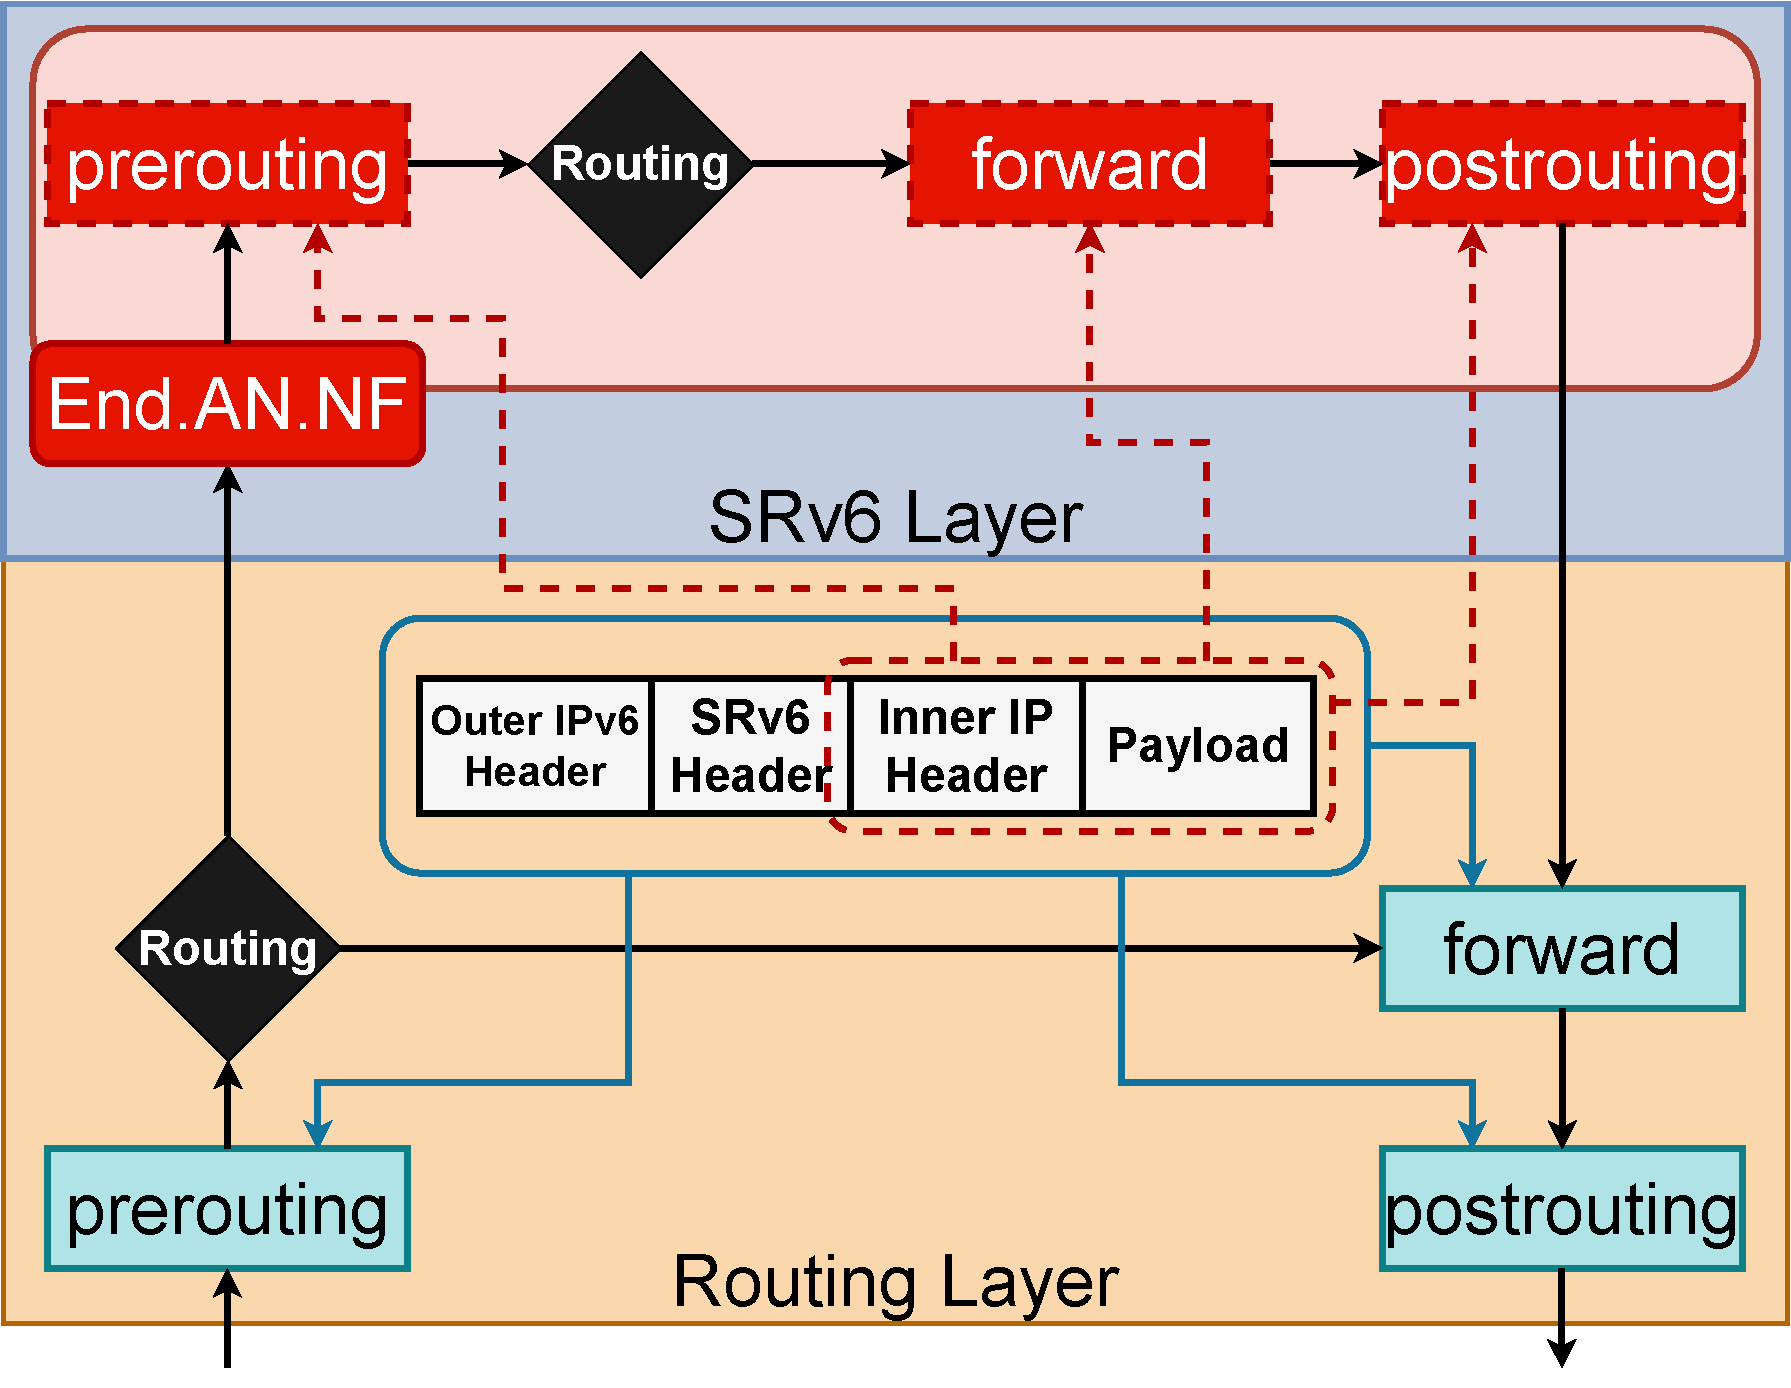
\includegraphics[
      width=0.95\linewidth,
      keepaspectratio=true
    ]{img/End-AN-NF-hooks.pdf}
    \caption{\texttt{End.AN.NF} applies three netfilter hook points, prerouting, forward, and postrouting, to inner packets encapsulated in SRv6.}
    \label{fig:hooks}
  \end{figure}
  
  \begin{algorithm*}[t]
    \caption{Pseudo code of passing a packet to a netfilter hook point in \texttt{End.AN.NF}}
    \small
    \label{alg:end-an-nf}
    \begin{algorithmic}[1]
      \if 0
      \Function {Process\_End.AN.NF}{$packet$}
      \State Call function \textbf{Pass\_to\_Hook} with following args: ($packet$, prerouting)
      \State Decrement segleft by 1
      \State Rewrite destination address based on the SID list and segleft, in the SID of the $packet$
      \State Lookup next hop in th routing table entry for rewrite new destination address
      \State Call function \textbf{Pass\_to\_Hook} with following args: ($packet$, forward)
      \State Call function \textbf{Pass\_to\_Hook} with following args: ($packet$, postrouting)
      \EndFunction
      \fi
      % \Function {Pass\_to\_Hook}{$packet$, $hook\_point$}
      \Function {PassPacketToHook}{$packet$}
      \If {the length of $ARG$ is specified for this \texttt{End.AN.NF} SID}
      \State Extract the $ARG$ value from the destination address of outer SRH
      \State Mark the $ARG$ value on the packet buffer $packet$
      \EndIf
      \State Switch the head of packet buffer $packet$ from the outer SRH to the inner packet
      \State Pass $packet$ to a netfilter hook
      \State Switch the head of packet buffer $packet$ from the inner packet to the outer SRH
      \EndFunction
    \end{algorithmic}
  \end{algorithm*}
  
  \begin{figure*}[t]
    \centering
    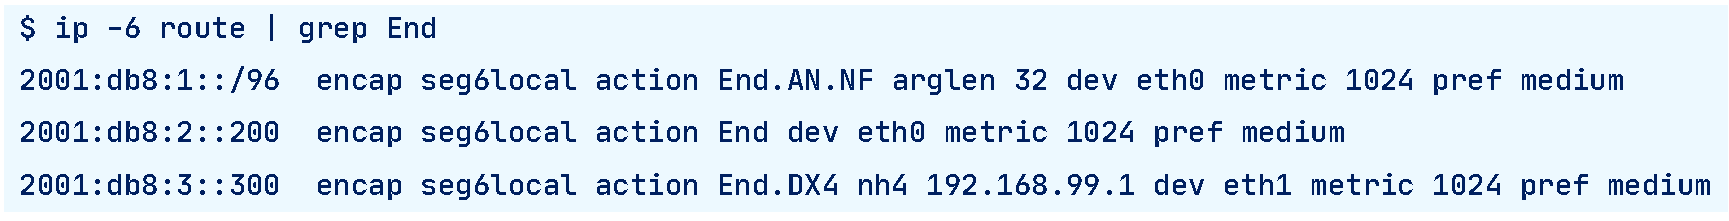
\includegraphics[width=0.95\linewidth]{img/End-FW-show-route.pdf}
    \caption{The modified Linux kernel treats an \texttt{End.AN.NF} SID as an IPv6 routing table entry. We can manage the \texttt{End.AN.NF} routes with the existing tools such as iproute2.}
    \label{fig:show-route}
  \end{figure*}

\section{実装}
\label{section:implementation}
End.AN.NF は Linux カーネルで動作する SRv6 ビヘイビアである.
End.AN.NF を実装するためには,Linux カーネルの SRv6 の実装を理解する必要がある.
本セクションでは,End.AN.NF 自体の実装を解説しながら Linux カーネルにおける SRv6 の実装についても述べる.
また,本研究では linux-5.15.106 を対象として End.AN.NF を実装する.
ビルド時のカーネルコンフィグを付録としてとして本論文末尾に掲載する.
本提案手法実装に利用した Linux フレーバーは,ubuntu のミニマムカスタムイメージである.
カーネルコンフィグを編集し,動作に必要なネットワークドライバや VRF カーネルモジュールなどを有効にしている.
また,本実装の動作検証はコンテナ技術を利用して仮想的なトポロジを作成して行った.
コンテナを動作させるにあたり,mobyproject~\cite{moby} の提供するカーネルコンフィグのチェックツール~\cite{mobysh}を利用した.
また,オーディオや GPIO サポートなど,本研究の提案手法の実装及び動作検証,計測に必要のない項目は無効化している.


\subsection{Linux における SRv6 ビヘイビアの実装}
\label{sbsection:linux-packet-forwarding}
Linux における SRv6 End ビヘイビア や End.DT4 ビヘイビアなどの実装は主に,\texttt{net/ipv6/seg6local.c} に記述されている.
章~\ref{section:linux-and-netfilter} で述べたように,Linux はカーネルモジュールという仕組みを使うことで Linux のカーネルのコードそのものを書き換えないでも機能を追加実装することができる.
しかし,seg6local の実装についてはカーネルモジュールとして提供されておらず,Linux カーネルのソースコード内で直接 SRv6 ビヘイビアを実装する手法が取られているため,直接 Linux カーネルのプロトコルスタックの実装を変更する必要がある.


独自の SRv6 ビヘイビアを追加するためには,まず \texttt{net/ipv6/seg6local.c} で定義されている \texttt{seg6\_action\_table} の末尾に要素を追加する必要がある.
End.AN.NF を実装するために追加した記述を,ソースコード~\ref*{seg6-action-desc} として実際のコードを抜粋したものを示す.
この \texttt{seg6\_action\_table} は \texttt{seg6\_action\_desc} 構造体の配列である.
\texttt{seg6\_action\_desc} のフィールドについて,特筆するべきは \texttt{input} フィールド及び \texttt{slwt\_ops} フィールドである.
受信したパケットの宛先アドレスが自身の持つルーティングテーブル上で,1 つの SRv6 ビヘイビアとして表現されていた場合,そのパケットは Linux ネットワークスタックの SRv6 レイヤへ到達し,パケットは SRv6 ビヘイビア毎に固有の処理の実装に渡される.
\texttt{input} フィールドには,最初に渡される SRv6 ビヘイビア毎に固有の関数へのポインタが代入される.
ソースコード~\ref*{seg6-action-desc} では \texttt{input} フィールドに \texttt{input\_action\_end\_nf} 関数へのポインタが設定されている.この関数の実装については以降で解説する.
\texttt{slwt\_ops} フィールドには,SID と SRv6 ビヘイビアを経路情報としてルーティングテーブルに設定するときに呼びされる関数へのポインタが代入される.
例えば End.DT4 の実装では,\texttt{slwt\_ops} フィールドにはパケットから SRH をデカプセル化したあとにルックアップする VRF を指定するための処理が定義された関数が設定されている.
End.AN.NF の場合,SID の IPv6 アドレスの下位何 bit を \texttt{ARG} として利用するかを指定するための処理が定義された関数である \texttt{seg6\_end\_nf\_build} へのポインタが設定されている.

End.AN.NF は,SID 内部の \texttt{ARG} 部をパケットバッファに埋め込んだ上で,SRH でカプセル化された内部パケットに対して netfilter フックポイントを通過させる.
これらの処理は \texttt{input\_action\_end\_nf} 関数内で行われる.
ソースコード~\ref*{input-action1} に,\texttt{input\_action\_end\_nf} 関数内で SID 内部の \texttt{ARG} 部をパケットバッファに埋め込む部分の処理を示す.
\texttt{slwt} は \texttt{seg6\_local\_lwt} 構造体へのポインタであり,これは \texttt{input\_action\_end\_nf} 関数呼び出し時に引数として渡される.
\texttt{seg6\_local\_lwt} 構造体には SRv6 ビヘイビアの動作に必要な様々なのフィールドが定義されいている.
パケットが入ってきたインターフェースを表す数値や,End.DT4 などで使うためのルーティングテーブル ID などが含まれている.
End.AN.NF の実装のために,\texttt{seg6\_local\_lwt} 構造体へ \texttt{\_\_u8} 型の \texttt{arg\_len} というフィールドを追加した.
このフィールドは SID の \texttt{ARG} 部分の長さを示しており,このフィールドはソースコード~\ref*{seg6-action-desc} の \texttt{slwt\_ops} フィールドに設定された \texttt{seg6\_end\_nf\_build} 関数によって設定される.
mark の計算及びパケットバッファへの埋め込みは,\texttt{ARG} が定義されているときにのみ行う.
End.AN.NF において,\texttt{ARG} フィールドの利用は任意である.
\texttt{ARG} を利用してパケットバッファにマークを付ける必要がない場合,SID を定義する際に \texttt{ARG} の長さを $0$ とすることで \texttt{ARG} は無効になる.
なお,\texttt{ARG} の長さを負の値にすることはできない.
Linux では,ユーザ空間からカーネルが管理するルーティングテーブルにエントリーを追加する際,NETLINK メッセージでやり取りをする.
End.AN.NF の SID を経路表に追加する際,特定のフォーマットで NETLINK メッセージを作成する.
そのメッセージの中には \texttt{ARG} の流さを指定するフィールドが定義されており,受け取ったメッセージは \texttt{seg6\_end\_nf\_build} 関数内でバリデートされ,\texttt{ARG} の長さが負だった場合は経路情報としてルーティングテーブルに載らない.
ソースコード~\ref*{input-action1} では,\texttt{arg\_len} が $0$ でない,すなわち \texttt{ARG} が有効であるときに if 文内部の処理が実行される.
計算された結果は Linux 上のパケットバッファを示す \texttt{sk\_buff} 構造体の mark フィールドに設定される.

\texttt{input\_action\_end\_nf} 関数の中で,SRH でカプセル化されたパケットを実際に netfilter フックポイントへ通過させている処理を抜粋したコードを,ソースコード~\ref*{input-action2} として示す.
End.AN.NF は,SRv6 パケットの SRH 部分を隠蔽して netfilter にパケットを通す.
ソースコード~\ref*{input-action2} の中で,SRH を隠蔽する,という処理は \texttt{skb\_pull} 関数と \texttt{skb\_reset\_network\_header} 関数の呼び出しによって実現される.
先に述べた通り,Linux カーネルではパケットバッファを \texttt{sk\_buff} 構造体で管理している.
Linux カーネルでパケットバッファを参照して各ネットワークレイヤでパケット転送処理を実行する際,処理ごとに \texttt{sk\_buff} 構造体内部の \texttt{head} ポインタを進める必要がある.
\texttt{head} ポインタは,パケットバファの中で現在処理をしているポインタの位置を示すものである.
例えば,Ether レイヤの処理をしているときはこのポインタは Ether フレームの先頭を指す.
Ether レイヤの処理が終わったあとは,\texttt{head} ポインタの位置を次のレイヤ,カプセル化されていない一般的なパケットであれば IP レイヤへずらす.
通常このように \texttt{head} ポインタの位置を進める場合は,\texttt{skb\_pull} 関数を利用する.
\texttt{skb\_pull} 関数の第一引数は \texttt{sk\_buff} 構造体へのポインタであり,第二引数はどれだけ進めるかを整数値で渡す.
ソースコード~\ref*{input-action2} では,第二引数に \texttt{offset} という変数を渡している.
この変数には,予め SRH の先頭から内部パケットのヘッダまでの長さを計算して代入してある.
\texttt{skb\_pull} 関数の呼び出し後は,\texttt{skb\_reset\_network\_header} 関数を使用することで,IP レイヤのヘッダ位置を再度アップデートする.

ソースコード~\ref*{input-action2} の 9 行目から 11 行目は実際に SRH でカプセル化された内部パケットを prerouting フックポイントへ通過させている処理である.
netfilter フックポイントへの通過は,\texttt{NF\_HOOK} マクロを呼び出すことで実現できる.
netfilter フックポイントを通過させた後は \texttt{skb\_push} 関数を呼び出しており,この関数は \texttt{skb\_pull} 関数とは対象的に指定した分 \texttt{head} ポインタを前に戻す関数である.
\texttt{skb\_push} 関数の呼び出し後は,\texttt{skb\_pull} 関数呼び出し時と同様に \texttt{skb\_reset\_network\_header} 関数を呼び出してヘッダの位置をもとに戻している.

ソースコード~\ref*{input-action2} の 19 行目,及び 21 行目では,SRv6 End ビヘイビアに対応する処理を行っている.
\texttt{advance\_nextseg} 関数は,segleft をデクリメントして宛先アドレスを新たな SID で書き換える処理を行う関数である.
また,\texttt{seg6\_lookup\_nexthop} 関数では,新たな SID で書き換えた宛先アドレスに対するネクスホップを決定している.
SRv6 End ビヘイビアが行う転送処理はこの大きく分けてこの 2 つであり,この転送処理は一般的なパケット転送処理とは異なる.
そのため,SRH でカプセル化された内部パケットにとってのフォワード操作,netfilter の forward フックポイントを適用するタイミングには議論の余地がある.
本研究では,segleft のデクリメントと新たな SID による宛先アドレスの更新,及び新たな宛先アドレスのネクストホップの決定を,SRH でカプセル化された内部パケットにとってのフォワード操作として解釈し実装する.

ソースコード~\ref*{input-action2} の 26 行目,及び 27 行目では,ソースコード~\ref*{input-action1} と同じように \texttt{ARG} の値をパケットバッファのマークフィールドに設定している.
パケットバッファのマークフィールドは,End.AN.NF に限らず,汎用的に利用されるフィールドである.
汎用的であるため,netfilter-based アプリケーションからその値を参照して処理内容を変えることができる.
ただし,その反面汎用的であるがゆえに他の用途で利用されたり,値が書き換わったりすることがある.
よって,ここでは forward フックポイントを通過する前に再度マークを付け直している.
パケットを forward フックポイントへ通過させる処理以降は,ほとんど同じ処理でパケットを同様に postrouting フックポイントへ通過させる.

ソースコード~\ref*{input-action2} に示すように,SRv6 パケットに対して End.AN.NF を使って SRH でカプセル化された内部パケットを netfilter フックポイントへ通過させる処理は非常に単純である.
処理の殆どがポインタの加算及び減算になるように考慮しており,オーバーヘッドがなるべく小さくなるようにしている.


\begin{lstlisting}[caption=Add definition of End.AN.NF to seg6\_action\_table,label=seg6-action-desc]
static struct seg6_action_desc seg6_action_table[] = {
  .
  .
  .
  // その他のビヘイビアの定義
  {
    .action   = SEG6_LOCAL_ACTION_END_NF,
    .attrs    = SEG6_F_ATTR(SEG6_LOCAL_NF),
    .optattrs = SEG6_F_LOCAL_COUNTERS,
    .input    = input_action_end_nf,
    .slwt_ops = {
        .build_state = seg6_end_nf_build,
    },
  },
};
\end{lstlisting}

\begin{lstlisting}[caption=Set a mark to a packet buffer,label=input-action1]
static int input_action_end_fw(struct sk_buff *skb,
  			struct seg6_local_lwt *slwt)
{
  .
  .
  .
  if (slwt->arg_len) {
    memcpy(&daddr_segment, &outer_header->daddr.s6_addr32[3], sizeof(daddr_segment));
    arg = ntohl(daddr_segment);
    mask = (1UL << slwt->arg_len) - 1;
    arg &= mask;
    skb->mark = arg;
  }
  .
  .
  .
}
\end{lstlisting}

\begin{figure*}[t]
\begin{lstlisting}[caption=Apply netfilter to SRv6 inner packet,label=input-action2]
static int input_action_end_fw(struct sk_buff *skb,
        struct seg6_local_lwt *slwt)
{
  .
  .
  .
  skb_pull(skb, offset);
  skb_reset_network_header(skb);
  ret = NF_HOOK(NFPROTO_IPV4, NF_INET_PRE_ROUTING,
        dev_net(skb->dev), NULL, skb, skb->dev,
        skb_dst(skb)->dev, dummy_okfn);

  skb_push(skb, offset);
  skb_reset_network_header(skb);

  if (ret != 1)
    return ret;

  advance_nextseg(srh, &ipv6_hdr(skb)->daddr);

  seg6_lookup_nexthop(skb, NULL, 0);

  skb_pull(skb, offset);
  skb_reset_network_header(skb);

  if (slwt->arg_len)
    skb->mark = arg;
  ret = NF_HOOK(NFPROTO_IPV4, NF_INET_FORWARD,
        dev_net(skb_dst(skb)->dev), NULL, skb, skb->dev,
        skb_dst(skb)->dev, dummy_okfn);
  if (ret != 1) {
    skb_push(skb, offset);
    skb_reset_network_header(skb);
    return ret;
  }

  if (slwt->arg_len)
    skb->mark = arg;

  ret = NF_HOOK(NFPROTO_IPV4, NF_INET_POST_ROUTING,
        dev_net(skb->dev), NULL, skb, skb->dev,
        skb_dst(skb)->dev, dummy_okfn);

  skb_push(skb, offset);
  skb_reset_network_header(skb);

  if (ret != 1)
    return ret;

  return dst_input(skb);
  .
  .
  .
}
  \end{lstlisting}
\end{figure*}